% bare_jrnl.tex
% V1.4b
% 2015/08/26
% by Michael Shell
% see http://www.michaelshell.org/
% for current contact information.                                                                 
%%%%%%%%%%%%%%%%%%%%%%%%%%%%%%%%%%%%%%%%%%%%%%%%%%%%%%%%%%%%%%%%%%%%

%% This is a skeleton file demonstrating the use of IEEEtran.cls
%% (requires IEEEtran.cls version 1.8b or later) with an IEEE
%% journal paper.
%%
%% Support sites:
%% http://www.michaelshell.org/tex/ieeetran/
%% http://www.ctan.org/pkg/ieeetran
%% and
%% http://www.ieee.org/


\documentclass[journal]{IEEEtran}

\usepackage{circuitikz}          % antes de babel
\usepackage{tikz}
\usepackage[spanish, es-noshorthands]{babel}
\usepackage{float}
\usepackage{instructivo}
\graphicspath{{./}{./fig/}}
\usepackage[natbib=true,style=trad-unsrt,backend=biber]{biblatex}
\addbibresource{literatura.bib}

\hyphenation{op-tical net-works semi-conduc-tor}

\usepackage{amsmath}
\usetikzlibrary{shapes, arrows.meta, positioning, calc}
 
% --- Estilos ---
\tikzset{
  block/.style={
    draw, rectangle,
    minimum width=3.2cm, minimum height=1.2cm,
    align=center, font=\small
  },
  line/.style={draw, -{Latex[length=2.5mm, width=2mm]}},
  siglabel/.style={font=\footnotesize, text=blue!65!black},
  blklabel/.style={font=\footnotesize, right=0.15cm, text=black}
}

\begin{document}
\setlength{\parindent}{4.2mm}
%
% paper title
% Titles are generally capitalized except for words such as a, an, and, as,
% at, but, by, for, in, nor, of, on, or, the, to and up, which are usually
% not capitalized unless they are the first or last word of the title.
% Linebreaks \\ can be used within to get better formatting as desired.
% Do not put math or special symbols in the title.
\title{Planta térmica TCLab}


\author{Matías~A.~Camacho,~\IEEEmembership{Estudiante,~TEC}
        y~Juan~P.~Elizondo,~\IEEEmembership{Estudiante,~TEC}
}


% The paper headers
\markboth{Laboratorio de control automático, IIS2026}%
{Laboratorio de control automático}


% make the title area
\maketitle



%%%%%%%%%%%%%%%%%%%%%%%%%%%%%%%%%%%%%%%%%%%%%%%%%%%%%%%%%%%%%%%%%%%%%%%%%%%%%%%%%%%%%%%%%%%%%%
%%%%%%%%%%%%%%%%%%%%%%%%%%%%%%%%%%%%%%%%%%%%%%%%%%%%%%%%%%%%%%%%%%%%%%%%%%%%%%%%%%%%%%%%%%%%%%
\section{Introducción}

\IEEEPARstart{E}{n}
%%%%%%%%%%%%%%%%%%%%%%%%%%%%%%%%%%%%%%%%%%%%%%%%%%%%%%%%%%%%%%%%%%%%%%%%%%%%%%%%%%%%%%%%%%%%%%
%%%%%%%%%%%%%%%%%%%%%%%%%%%%%%%%%%%%%%%%%%%%%%%%%%%%%%%%%%%%%%%%%%%%%%%%%%%%%%%%%%%%%%%%%%%%%%
\section{Resultados}
\begin{table}[H]
    \centering
    \caption{Validación cruzada del modelo FOPDT, modelo escalón frente a datos multinivel}
    \label{tab:validacion_fopdt}
    \begin{tabular}{lc}
        \hline
        \textbf{Parámetro} & \textbf{Valor} \\
        \hline
        $K$ & $0.937801~^\circ\mathrm{C}/\%$ \\
        $\tau$ & $189.293~\mathrm{s}$ \\
        $\theta$ & $21.001~\mathrm{s}$ \\
        RMSE & $1.2273~^\circ\mathrm{C}$ \\
        $R^2$ & $0.99175$ \\
        Ajuste & $90.92\%$ \\
        \hline
    \end{tabular}
\end{table}

\begin{figure}[H]
        \centering
        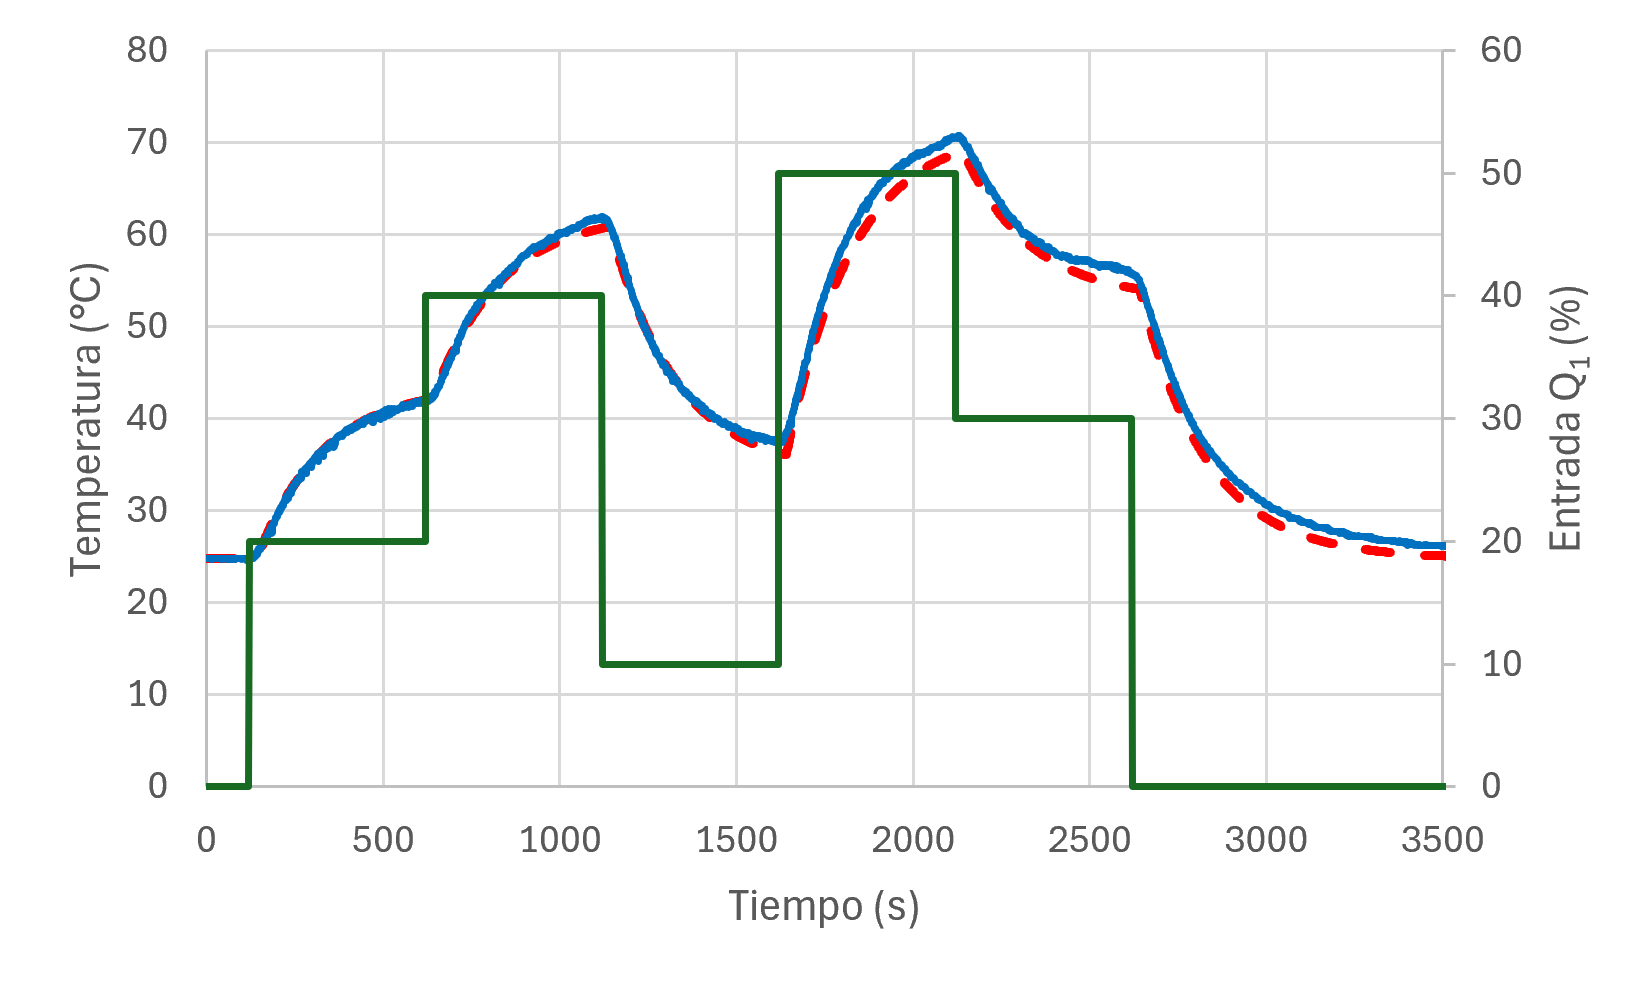
\includegraphics[width=0.8\linewidth]{ValCruzadaMultiescalonConFOPDTdeEscalon.png}
        \caption{Validación cruzada del modelo FOPDT, modelo escalón frente a datos multinivel}
        \label{fig:j}
\end{figure}

\begin{figure}[H]
        \centering
        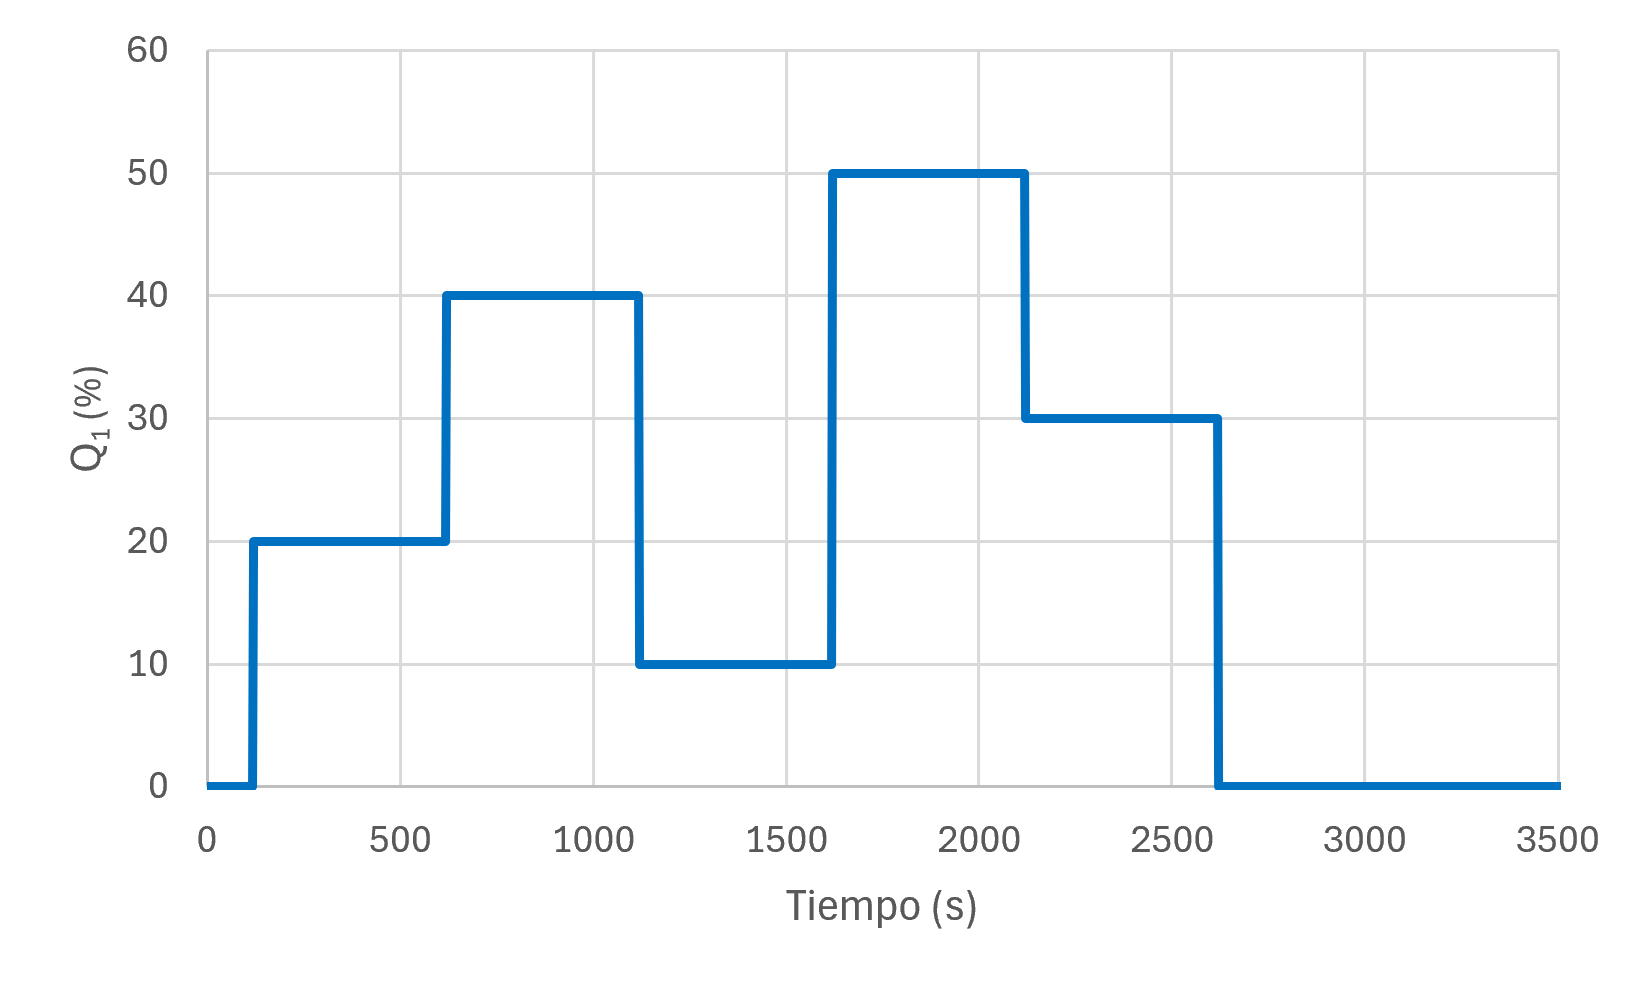
\includegraphics[width=0.8\linewidth]{Escalones.png}
        \caption{Entradas tipo escalón aplicadas al sistema}
        \label{fig:jj}
\end{figure}

\begin{figure}[H]
        \centering
        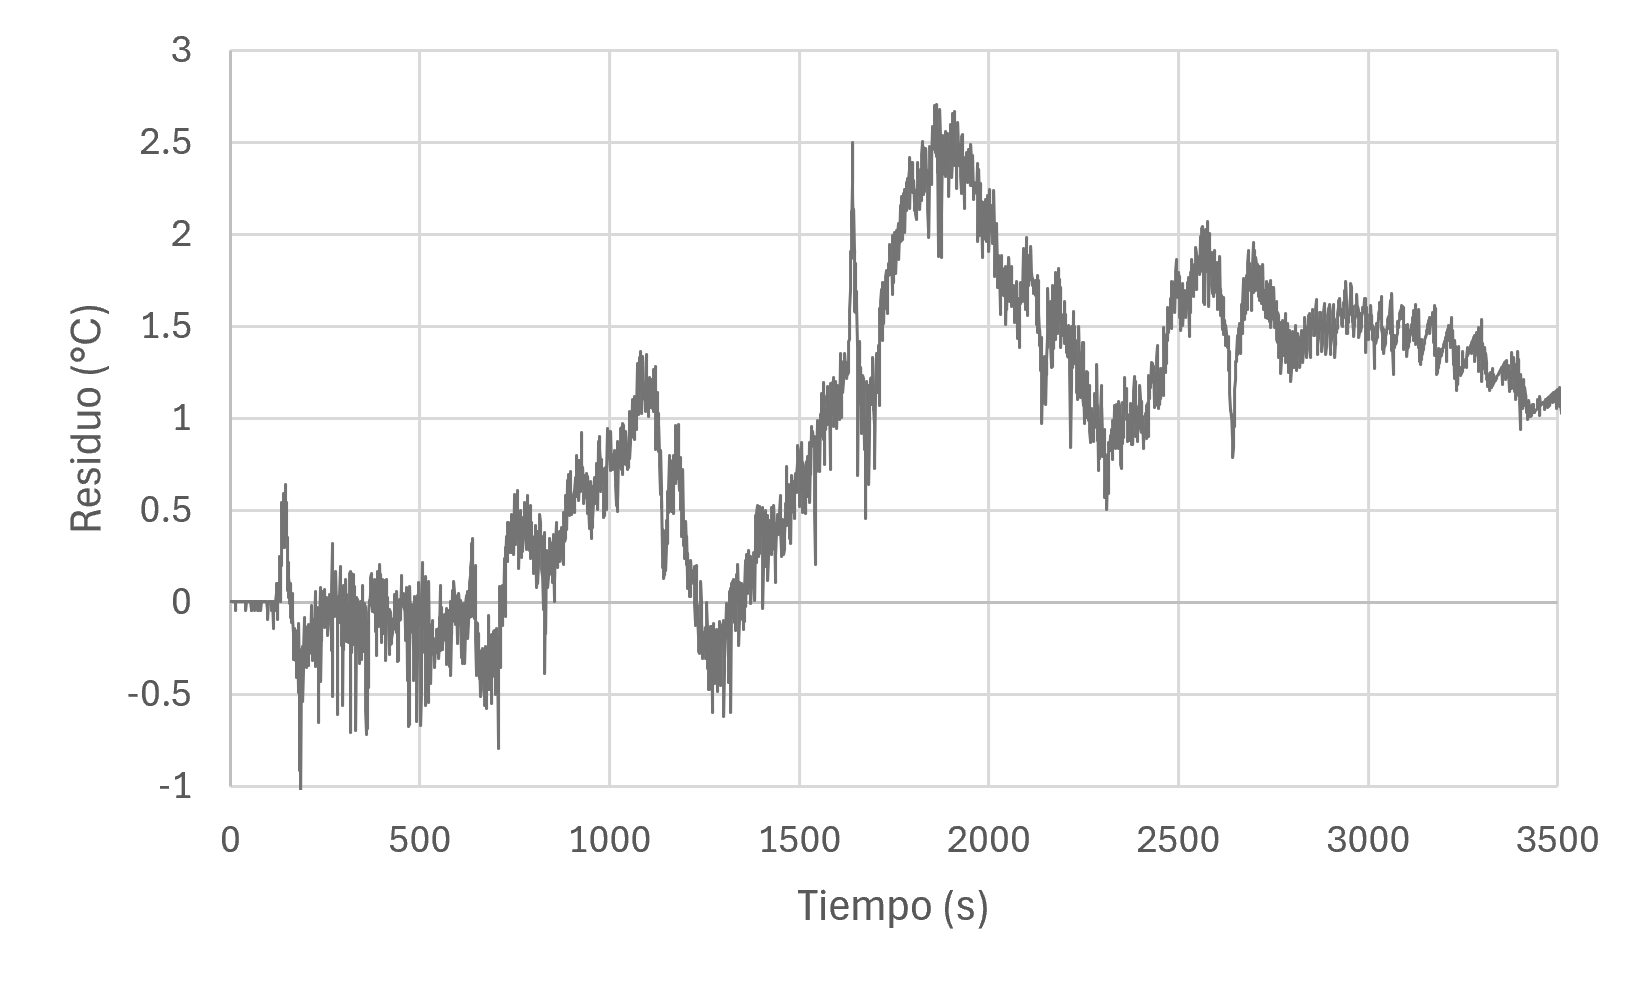
\includegraphics[width=0.8\linewidth]{ResiduoValCruzadaMultiescalonConFOPDTdeEscalon.png}
        \caption{Residuo de la validación cruzada del modelo FOPDT, modelo escalón frente a datos multinivel}
        \label{fig:jjj}
\end{figure}

\begin{table}[H]
    \centering
    \caption{Validación cruzada del modelo FOPDT, modelo multinivel frente a datos escalón}
    \label{tab:validacion_fopdt2}
    \begin{tabular}{lc}
        \hline
        \textbf{Parámetro} & \textbf{Valor} \\
        \hline
        $K$ & $0.980642~^\circ\mathrm{C}/\%$ \\
        $\tau$ & $208.731~\mathrm{s}$ \\
        $\theta$ & $13.000~\mathrm{s}$ \\
        RMSE & $1.7692~^\circ\mathrm{C}$ \\
        $R^2$ & $0.97211$ \\
        Ajuste & $83.30\%$ \\
        \hline
    \end{tabular}
\end{table}
\begin{figure}[H]
        \centering
        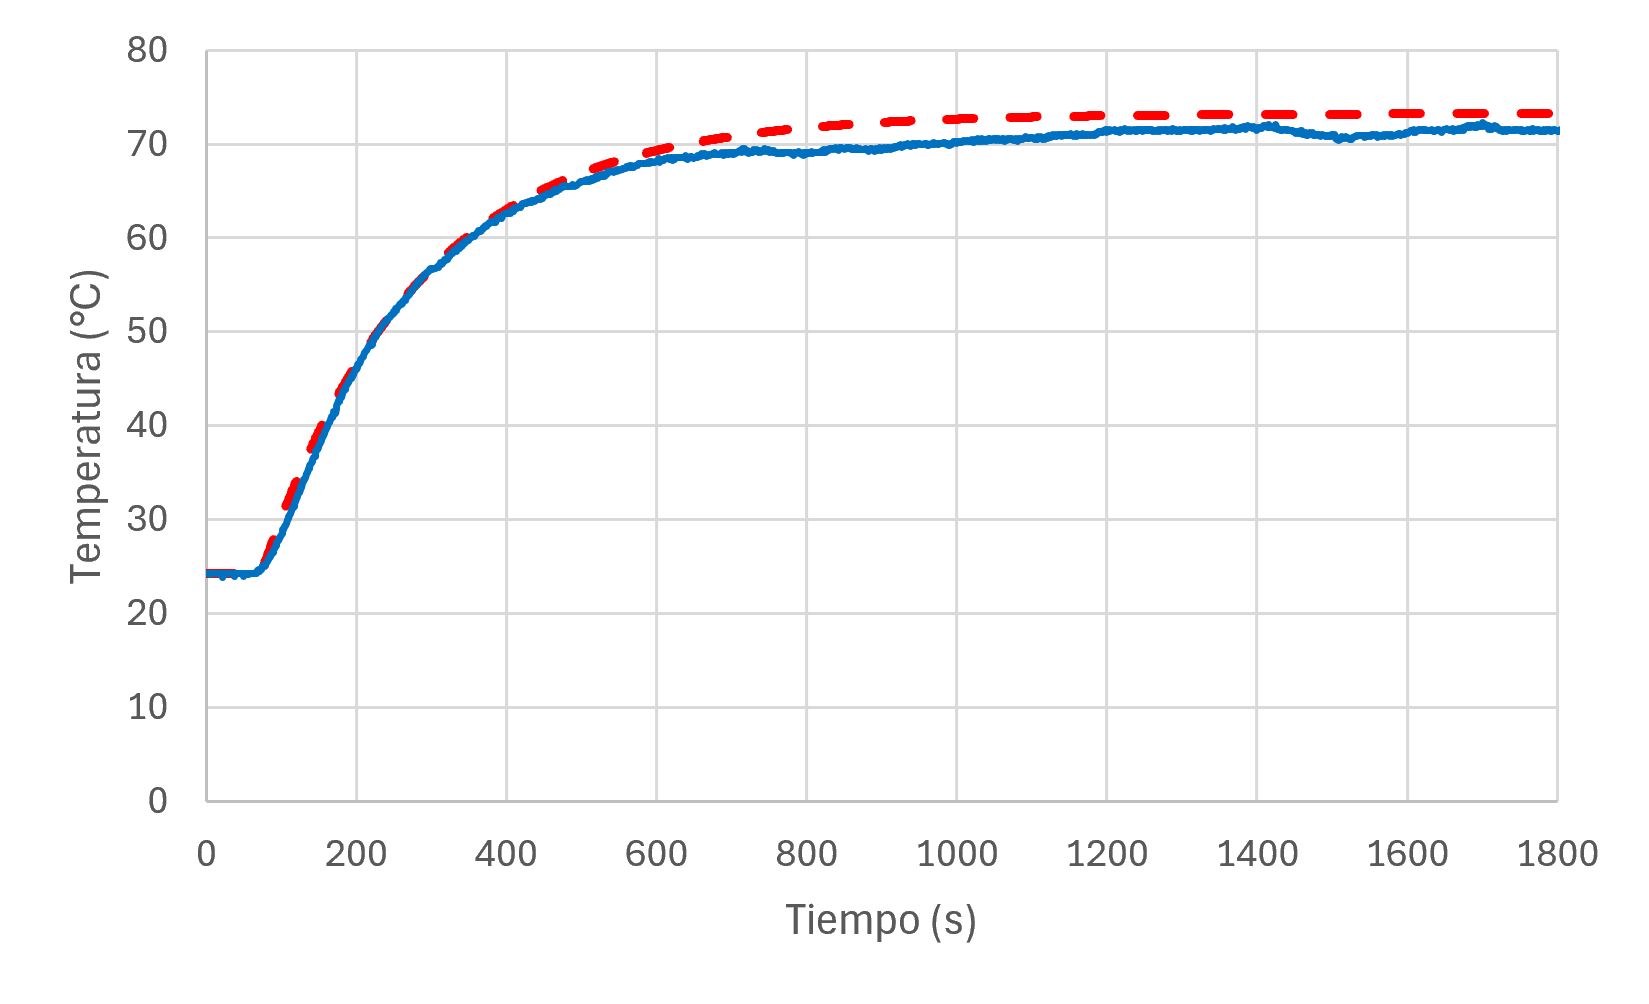
\includegraphics[width=0.8\linewidth]{ValCruzadaEscalonConFOPDTdeMultiescalon.png}
        \caption{Validación cruzada del modelo FOPDT, modelo multinivel frente a datos escalón}
        \label{fig:k}
\end{figure}

\begin{figure}[H]
        \centering
        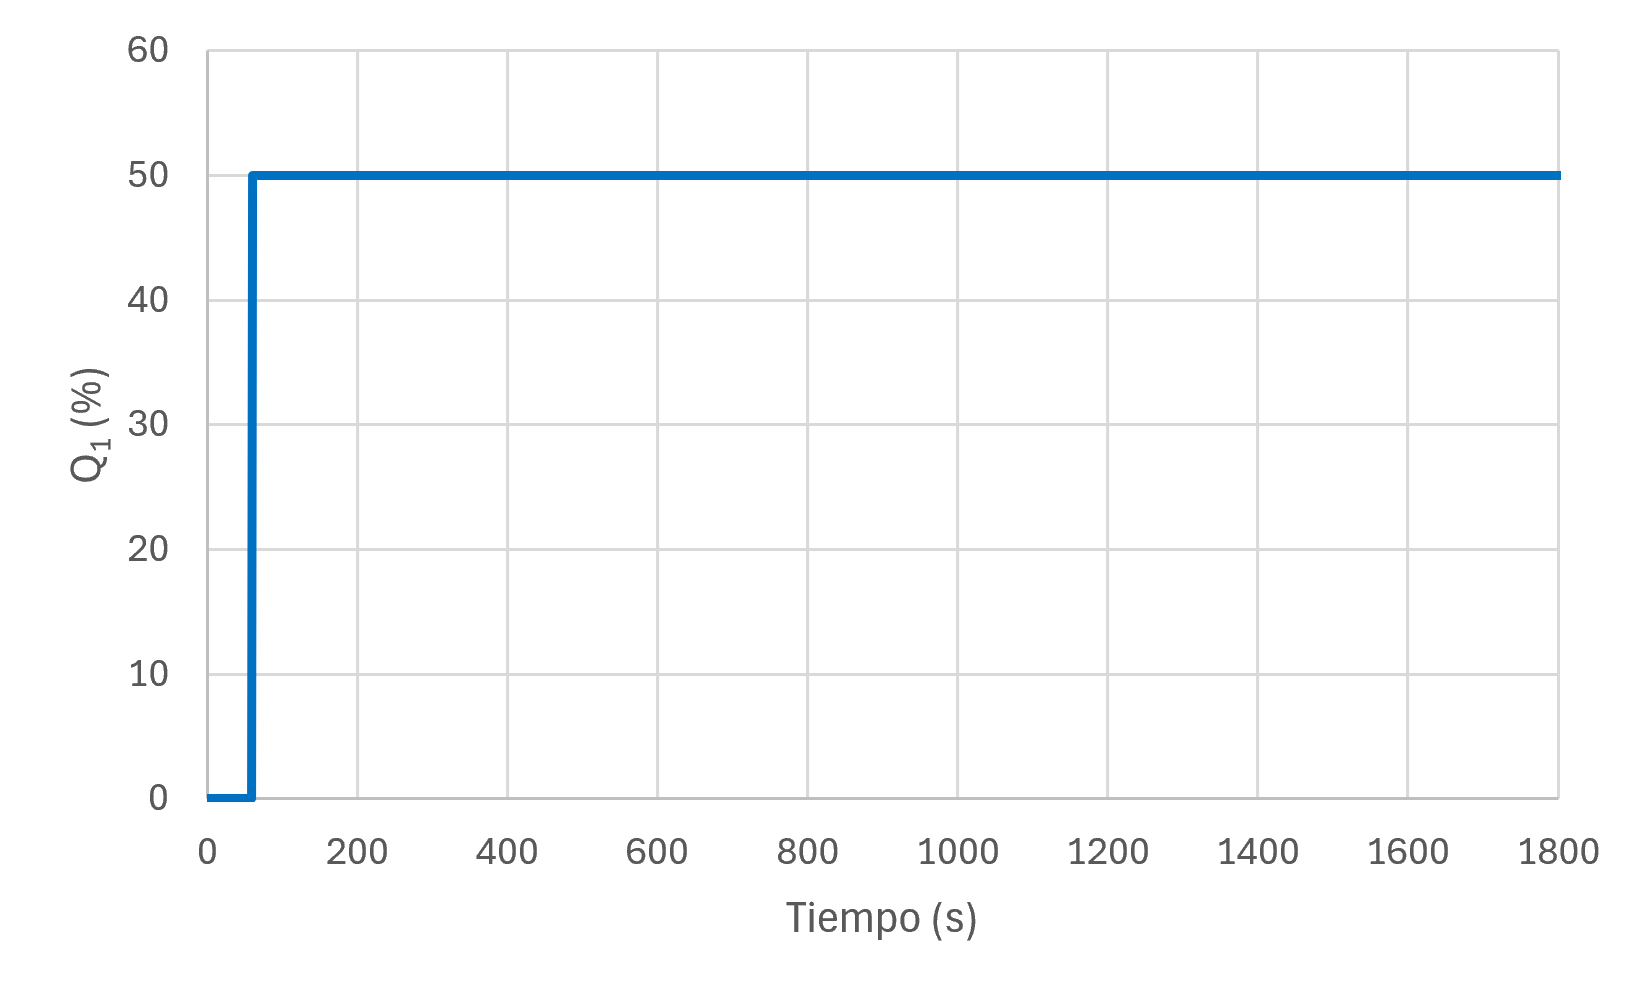
\includegraphics[width=0.8\linewidth]{Escalon.png}
        \caption{Entradas tipo escalón aplicadas al sistema}
        \label{fig:kk}
\end{figure}

\begin{figure}[H]
        \centering
        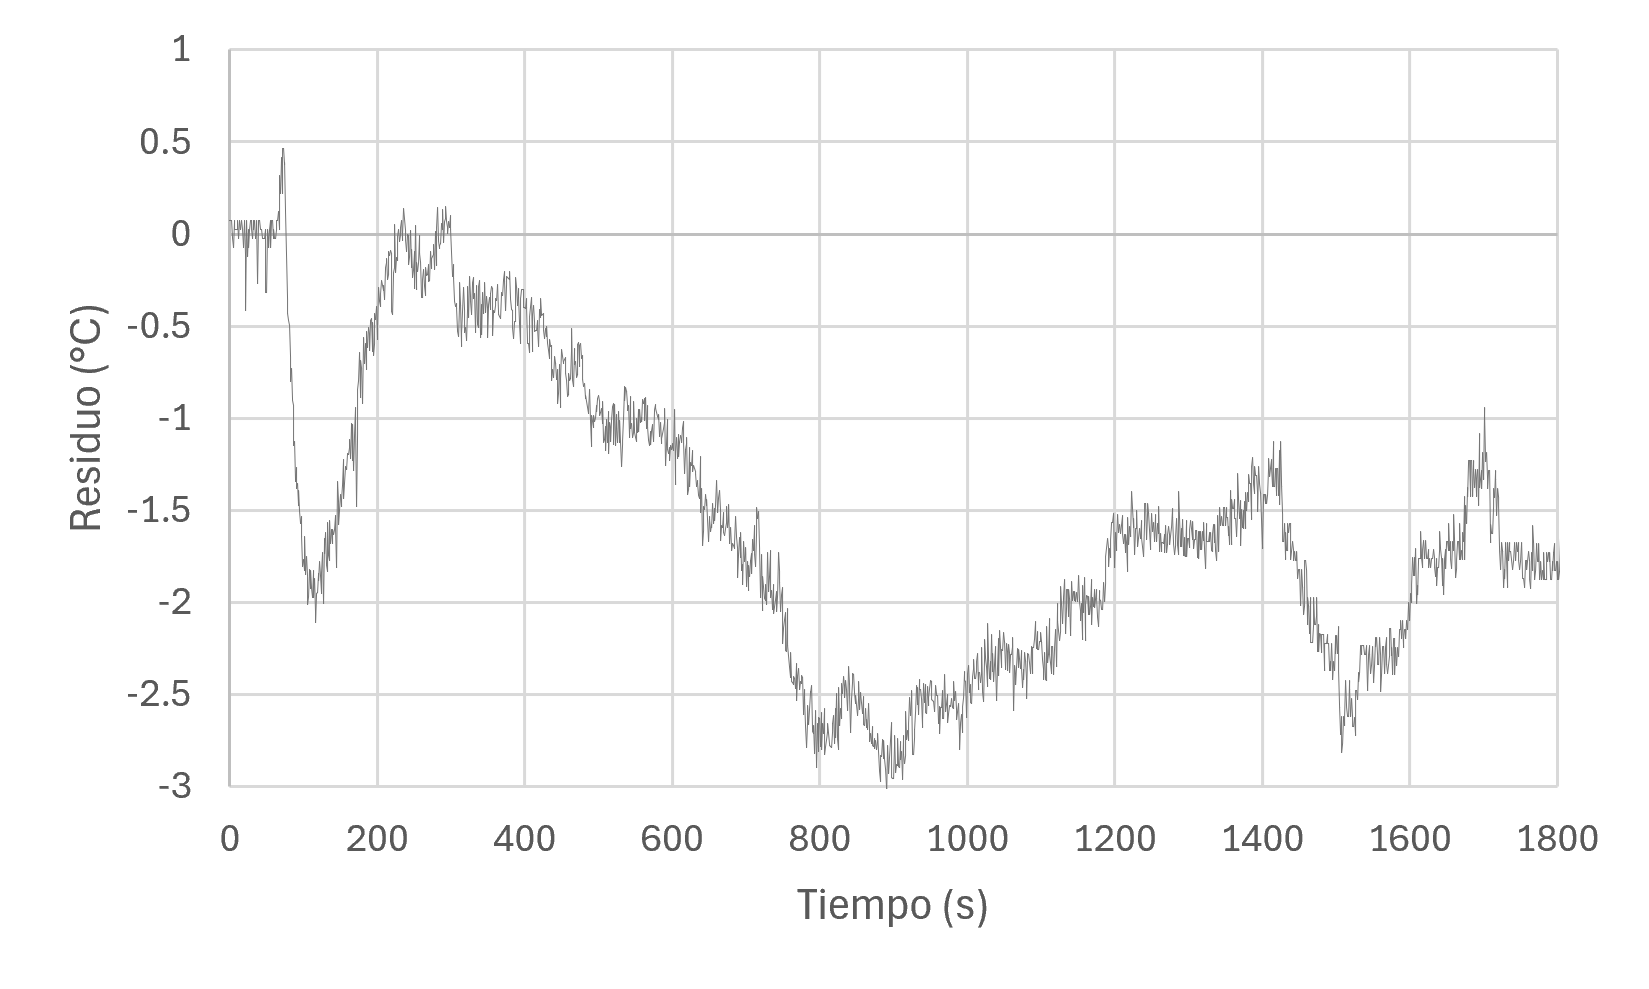
\includegraphics[width=0.8\linewidth]{ResiduoValCruzadaEscalonConFOPDTdeMultiescalon.png}
        \caption{Residuo de la validación cruzada del modelo FOPDT, modelo multinivel frente a datos escalón}
        \label{fig:kkk}
\end{figure}

\subsection{Selección del modelo nominal de la planta}
Basándose en los resultados obtenidos de la validación cruzada, se escoje el modelo FOPDT basado en los datos experimentales 
de la prueba con un escalón. Esto debido al alto porcentaje de ajuste y valor de $R^2$ muy cercano a 1. Además, el modelo fue capaz de predecir muy bien el comportamiento del sistema 
ante varios tipos de entradas. El mmodelo FOPDT basado en los datos del experimento multinivel presentó un ajuste más alejado al 100\% y con un valor de $R^2$ más lejano a 1.

Analizando las gráficas de residuos \ref{fig:jjj} y \ref{fig:kkk}, ambos modelos muestran picos alredor de $\pm1^\circ\text{C}$ y $\pm3^\circ\text{C}$.

Sin embargo, es importante mencionar que la validación cruzada con datos multinivel utilizando el modelo FOPDT de una entrada escalón no tuvo la misma capacidad predictiva para todas las entradas multiescalón. Como se puede ver en la gráfica \ref{fig:j}, el modelo no predijo con tanta exactitud luego de la entrada de 50\%. Aun así, ambos modelos tienen buenas capacidades para predecir el comportamiento del sistema, por lo que la elección del FOPDT basado en los datos 
del experimento con escalón da seguridad de que el modelo es capaz de predecir distintas entradas con bastante exactitud. 

Por consiguiente, el modelo escogido es el siguiente (véase unidades en la tabla \ref{tab:validacion_fopdt}).

\begin{equation}
        G_{p,nom}(s)=\frac{K_{nom}e^{-\theta s}}{\tau s + 1}=\frac{0.937801e^{-21s}}{189.293s+1}
\end{equation}

%%%%%%%%%%%%%%%%%%%%%%%%%%%%%%%%%%%%%%%%%%%%%%%%%%%%%%%%%%%%%%%%%%%%%%%%%%%%%%%%%%%%%%%%%%%%%%
%%%%%%%%%%%%%%%%%%%%%%%%%%%%%%%%%%%%%%%%%%%%%%%%%%%%%%%%%%%%%%%%%%%%%%%%%%%%%%%%%%%%%%%%%%%%%%
\section{Diseño del controlador PI}
Para diseñar el controlador PI, se utilizó como referencia la siguiente ecuación
\begin{equation}
        G_{c}(s)=K_p+\frac{K_i}{s}=K_p\left(1+\frac{1}{T_i s}\right)
\end{equation}

donde
\begin{equation}
        K_i=\frac{K_p}{T_i}
\end{equation}

Además, siguiendo reglas SIMC, se tiene que
\begin{equation}
        K_p=\frac{1}{K}\frac{\tau}{\tau_c+\theta}
\end{equation}

\begin{equation}
        T_i=\min\{\tau,4(\tau_c+\theta)\}
\end{equation}

\begin{equation}
        K_i=\frac{K_p}{T_i}
\end{equation}

Por ende, el parámetro $\tau_c$ es el único que se decide para la sintonización. Se utilizará como primera configuración $\tau_c=2\theta$

Se obtienen los siguientes resultados.

\begin{table}[H]
    \centering
    \caption{Modelo nominal y parámetros del controlador PI-SIMC}
    \label{tab:parametros_controlador}
    
    \resizebox{\columnwidth}{!}{%
    \begin{tabular}{
        >{\centering\arraybackslash}p{1.5cm}
        >{\centering\arraybackslash}p{1.5cm}
        >{\centering\arraybackslash}p{2cm}
        >{\centering\arraybackslash}p{2.2cm}
    }
        \hline
        \textbf{Parámetro de la planta} & \textbf{Valor} &
        \textbf{Parámetro del controlador} & \textbf{Valor} \\
        \hline
        $K$&$0.937801\,^\circ\mathrm{C}/\%$&$\tau_c$ &$42\,\mathrm{s}$ \\
        $\tau$&$189.293\,\mathrm{s}$   & $K_p$ & $3.203932\,^\circ\mathrm{C}/\%$ \\
        $\theta$ &$21\,\mathrm{s}$  & $T_i$ & $84.004\,\mathrm{s}$ \\
        & & $K_i$ & $0.016926\,^\circ\mathrm{C}/(\% \mathrm{s})$ \\
        \hline
    \end{tabular}%
    }
\end{table}

\begin{equation}
        G_{c}(s)=3.20\left(1+\frac{1}{84.004 s}\right)
\end{equation}

\section{Análisis y Validación}

%%%%%%%%%%%%%%%%%%%%%%%%%%%%%%%%%%%%%%%%%%%%%%%%%%%%%%%%%%%%%%%%%%%%%%%%%%%%%%%%%%%%
%%%%%%%%%%%%%%%%%%%%%%%%%%%%%%%%%%%%%%%%%%%%%%%%%%%%%%%%%%%%%%%%%%%%%%%%%%%%%%%%%%%%
\section{Conclusiones}

%%%%%%%%%%%%%%%%%%%%%%%%%%%%%%%%%%%%%%%%%%%%%%%%%%%%%%%%%%%%%%%%%%%%%%%%%%%%%%%%%%%%
%%%%%%%%%%%%%%%%%%%%%%%%%%%%%%%%%%%%%%%%%%%%%%%%%%%%%%%%%%%%%%%%%%%%%%%%%%%%%%%%%%%%


\printbibliography

%%%%%%%%%%%%%%%%%%%%%%%%%%%%%%%%%%%%%%%%%%%%%%%%%%%%%%%%%%%%%%%%%%%%%%%%%%%%%%%%%%%%
%%%%%%%%%%%%%%%%%%%%%%%%%%%%%%%%%%%%%%%%%%%%%%%%%%%%%%%%%%%%%%%%%%%%%%%%%%%%%%%%%%%%
\section{Biografías de los autores}

 
\begin{IEEEbiographynophoto}{Matías A. Camacho}
        Estudiante del Instituto Tecnológico de Costa Rica (TEC) en la carrera de ingeniería electrónica.
        
        Correo: jeacamacho@estudiantec.cr
\end{IEEEbiographynophoto}

\begin{IEEEbiographynophoto}{Juan P. Elizondo}
        Estudiante de Ingeniería Electrónica en el Tecnológico de Costa Rica (TEC).
        Cuenta con preparación y/o experiencia en áreas como:
        \begin{itemize}
            \item Arquitectura básica de redes, CISCO CCNA V7 (ITN), (2021).
            \item Fundamentos de ciberseguridad, CISCO Systems, (2022).
            \item Programa de tutorías estudiantiles, Tecnológico de Costa Rica, (2024).
            \item Diseño de circuitos digitales, TEC (2025).
        \end{itemize}
        
        Correo: juelizondo@estudiantec.cr
\end{IEEEbiographynophoto}


\vfill

\end{document}